\documentclass[answers]{exam}
\usepackage{marvosym}

%...TikZ & PGF
\usepackage{pgfplots}
\pgfplotsset{compat=1.11}
\tikzset{>=latex}
\usetikzlibrary{calc,math}
\usepackage{tikzsymbols}
\usepgfplotslibrary{fillbetween}
\usetikzlibrary{decorations.markings} 
\usetikzlibrary{arrows.meta} %...APP2 for arrows as objects and images
\usetikzlibrary{backgrounds} %...For shading portions of graphs
\usetikzlibrary{patterns} %...Unit 5 Problems
\usetikzlibrary{shapes.geometric} %...For drawing cylinders in Unit 2
\tikzset{
    mark position/.style args={#1(#2)}{
        postaction={
            decorate,
            decoration={
                markings,
                mark=at position #1 with \coordinate (#2);
            }
        }
    }
} %...See https://tex.stackexchange.com/questions/43960/define-node-at-relative-coordinates-of-draw-plot

\tikzset{
    declare function = {trajectoryequation10(\x,\vi,\thetai)= tan(\thetai)*\x - 10*\x^2/(2*(\vi*cos(\thetai))^2);},
    declare function = {trajectoryequation(\x,\vi,\thetai)= tan(\thetai)*\x - 9.8*\x^2/(2*(\vi*cos(\thetai))^2);},
    declare function = {patheq(\x,\yi,\vi,\thetai)= \yi + tan(\thetai)*\x - 9.8*\x^2/(2*(\vi*cos(\thetai))^2);},
    declare function = {patheqten(\x,\yi,\vi,\thetai)= \yi + tan(\thetai)*\x - 10*\x^2/(2*(\vi*cos(\thetai))^2);} %like patheq but with gravity = 10
}

%...siunitx
\usepackage{siunitx}
\DeclareSIUnit{\nothing}{\relax}
\def\mymu{\SI{}{\micro\nothing} }
\DeclareSIUnit\mmHg{mmHg}
\DeclareSIUnit{\mile}{mi}
%...NOTE: "The product symbol between the number and unit is set using the quantity-product option."

%...Other
\usepackage{amsthm}
\usepackage{amsmath}
\usepackage{amssymb}
\usepackage{cancel}
\usepackage{subcaption}
\usepackage{dashrule}
\usepackage{enumitem}
\usepackage{fontawesome}
\usepackage{multicol}
\usepackage{glossaries}
%\numberwithin{equation}{section}
\numberwithin{figure}{section}
\usepackage{float}
\usepackage{twemojis} %...twitter emojis
\usepackage{utfsym}
\newcommand{\R}{\mathbb{R}} %...real number symbol
\usepackage{graphicx}
\graphicspath{ {../Figures/} }
\usepackage{hyperref}
\hypersetup{colorlinks=true,
    linkcolor=blue,
    filecolor=magenta,
    urlcolor=cyan,}
\urlstyle{same}
\newcommand{\hdashline}{{\hdashrule{\textwidth}{0.5pt}{0.8mm}}}
\newcommand{\hgraydashline}{{\color{lightgray} \hdashrule{0.99\textwidth}{1pt}{0.8mm}}}

%...Miscellaneous user-defined symbols
\newcommand{\fnet}{F_{\text{net}}} %...For net force
\newcommand{\bvec}[1]{\vec{\mathbf{#1}}} %...bold vector
\newcommand{\bhat}[1]{\,\hat{\mathbf{#1}}} %...bold hat vector
\newcommand{\que}{\mathord{?}}  %...Question mark symbol in equation env
%...Define thick horizontal rule for examples:
\newcommand{\hhrule}{\hrule\hrule}
\let\oldtexttt\texttt% Store \texttt
\renewcommand{\texttt}[2][black]{\textcolor{#1}{\ttfamily #2}}% 

%...For use in the exam document class
\newif\ifprintmetasolutions


%...Decreases space above and below align and gather enironment
\makeatletter
\g@addto@macro\normalsize{%
  \setlength\abovedisplayskip{-3pt}
  \setlength\belowdisplayskip{6pt} 
}
\makeatother





\usepackage[margin=1in]{geometry}
\usepackage[figurewithin=none]{caption}
\usepackage{exam-randomizechoices}

\CorrectChoiceEmphasis{\color{red}\bfseries}
\renewcommand{\solutiontitle}{\noindent\textbf{\textcolor{red}{Solution:}}\enspace}

\usepackage{OutilsGeomTikz}
\usepackage{utfsym} %...Symbols in Unit 7 Problems
\usepackage{tabu} %...Symbols in Unit 7 Problems

%...For use in Unit 2            %    
\setlength{\columnsep}{2cm}      %
\setlength{\columnseprule}{1pt}  %
\usepackage[none]{hyphenat}      %
%%%%%%%%%%%%%%%%%%%%%%%%%%%%%%%%%

%...For use in Unit 11 on Waves:
\pgfdeclarehorizontalshading{visiblelight}{50bp}{  %
color(0.00000000000000bp)=(red);                   %
color(8.33333333333333bp)=(orange);                %
color(16.66666666666670bp)=(yellow);               %
color(25.00000000000000bp)=(green);                %
color(33.33333333333330bp)=(cyan);                 %
color(41.66666666666670bp)=(blue);                 %
color(50.00000000000000bp)=(violet)                %
}                                                  %

\newcommand{\checkbox}[1]{%
  \ifnum#1=1
    \makebox[0pt][l]{\raisebox{0.15ex}{\hspace{0.1em}\Large$\checkmark$}}%
  \fi
  $\square$%
}
%%%%%%%%%%%%%%%%%%%%%%%%%%%%%%%%%%%%%%%%%%%%%%%%%%%%

%...If using circuitikz package:
% \ctikzset{bipoles/battery1/height=0.5}
% \ctikzset{bipoles/battery1/width=0.25}
% \ctikzset{bipoles/resistor/height=0.15}
% \ctikzset{bipoles/resistor/width=0.4}
\usepackage{mdframed}

\setrandomizerseed{1}
\bracketedpoints
\addpoints

\newif\ifversionKlevel

\versionKleveltrue

\header{Physics L\\Test on Unit 4: Impulse and Work}{}{Name:\enspace\makebox[5cm]{\hrulefill}}

\ifversionKlevel
    \header{Physics K\\Test on Unit 4: Impulse and Work}{}{Name:\enspace\makebox[5cm]{\hrulefill}}
\fi

\begin{document}
\begin{questions}

\question 
Using the data in the table below, which object had the greatest change in momentum?

\begin{center}
    \begin{tabular}{|c|c|c|c|}
        \hline
        Object & Mass (kg) & Initial velocity (m/s) & Final velocity (m/s)\\ \hline
        Toy truck & 10 & 0 & 5\\ \hline
        Toy car & 5 & 0 & 5\\ \hline
    \end{tabular}
\end{center}

\begin{randomizechoices}[norandomize]
    \correctchoice The toy truck, because it has a larger mass but same change in velocity as the car.
    \choice The toy car, because it has a smaller mass but the same change in velocity as the toy truck.
    \choice Both have the same change in momentum because they both have the same change in velocity.
    \choice Neither. Both have a constant momentum.
\end{randomizechoices}

\question 
Which of the following representations of motion depicts an object with constant momentum?

\begin{center}
    \begin{tikzpicture}
        \begin{axis}[height=3.5cm,
            width=3.5cm,
            ymin=0,ymax=5,
            xmin=0,xmax=3,
            ticks=none,
            axis lines=left,
            ylabel={$v$},
            y label style={rotate=-90},
            xlabel={$t$},
            title={\ifprintanswers \color{red} \bfseries \fi Graph A},
        ]   
            \ifprintanswers
                \addplot[domain=0:2.5,very thick,red] {3};
            \else
                \addplot[domain=0:2.5,very thick] {3};
            \fi
        \end{axis}
    \end{tikzpicture}
    \hspace{2em}
    \begin{tikzpicture}
        \begin{axis}[height=3.5cm,
            width=3.5cm,
            ymin=0,ymax=5,
            xmin=0,xmax=3,
            ticks=none,
            axis lines=left,
            ylabel={$v$},
            y label style={rotate=-90},
            xlabel={$t$},
            title=Graph B,
        ]
            \addplot[domain=0:2,very thick,black] {4*x - x^2};
        \end{axis}
    \end{tikzpicture}
    \hspace{2em}
    \begin{tikzpicture}
        \begin{axis}[height=3.5cm,
            width=3.5cm,
            ymin=0,ymax=5,
            xmin=0,xmax=3,
            ticks=none,
            axis lines=left,
            ylabel={$v$},
            y label style={rotate=-90},
            xlabel={$t$},
            title={Graph C}
        ]
            \addplot[domain=0:2,very thick,black] {(x-2)^2};
        \end{axis}
    \end{tikzpicture}
    \hspace{2em}
    \begin{tikzpicture}
        \begin{axis}[height=3.5cm,
            width=3.5cm,
            ymin=0,ymax=5,
            xmin=0,xmax=3,
            ticks=none,
            axis lines=left,
            ylabel={$v$},
            y label style={rotate=-90},
            xlabel={$t$},
            title={Graph D}
        ]
            \addplot[domain=0:2.5,very thick,black] {1.5*x};
        \end{axis}
    \end{tikzpicture}
\end{center}

{\color{white} \tiny \vspace{-3em}
\begin{randomizeoneparchoices}[norandomize]
    \correctchoice \phantom{Graph A}
    \choice \phantom{Graph B}
    \choice \phantom{Graph C}
    \choice \phantom{Graph D}
\end{randomizeoneparchoices}
}

\question 
A student drops a \SI{2}{kg} textbook from rest from the second floor of the school. If the book reaches a velocity of \SI{14}{m/s} as it hits the ground, what is its change in momentum from the fall?

\begin{randomizechoices}[norandomize]
    \choice \SI{0}{kg\cdot m/s}
    \choice \SI{2}{kg\cdot m/s}
    \correctchoice \SI{28}{kg\cdot m/s}
    \choice \SI{14}{kg\cdot m/s}
\end{randomizechoices}

\question 
As the length of time 
%a given 
that a net force acts on an object increases, what must also increase?

\begin{randomizechoices}[norandomize]
    \choice The object's inertia
    \choice The frictional force acting on the object
    \correctchoice The change in momentum of the object
    \choice The reaction force acting on the object
\end{randomizechoices}

% \question
% The idea behind many types of collision safety equipment is to decrease the average force impacting the object being protected by

% \begin{randomizechoices}[norandomize]
%     \choice Decreasing the amount of time the force is applied to the object
%     \correctchoice Increasing the amount of time the force is applied to the object
% \end{randomizechoices}


\question
Engineers who build collision safety equipment are trying to make collisions safer passengers. The safety equipment does this by

\begin{randomizechoices}[norandomize]
    \choice decreasing the amount of time a force is applied to the object, which decreases the force.
    \choice decreasing the amount of time a force is applied to the object, which increases the force.
    \correctchoice increasing the amount of time a force is applied, which decreases the force.
    \choice increasing the amount of time a force is applied to the object, which increases the force.
\end{randomizechoices}

\clearpage
\question
The average net force shown in the graph below acts on a \SI{5}{kg} object for 10 seconds.

\begin{center}
    \begin{tikzpicture}
        \begin{axis}[width=6cm,height=4cm,
            xmin=0,xmax=10,
            ymin=0,ymax=5,
            axis lines=left,
            xlabel={Time (s)},
            ylabel={Force (N)},
            y label style={rotate=-90},
            xtick={0,1,...,10},
            ytick={0,1,...,5},
            grid=both,
        ]
            \draw[very thick] (0,3) -- ++(10,0);
        \end{axis}
    \end{tikzpicture}
\end{center}

What is the impulse on the object during this time period?

\begin{randomizechoices}[norandomize]
    \correctchoice \SI{30}{N\cdot s}
    \choice \SI{3}{N\cdot s}
    \choice \SI{15}{N\cdot s}
    \choice \SI{50}{N\cdot s}
\end{randomizechoices}

% What is the object's change in velocity during this time period?

% \begin{randomizechoices}[norandomize]
%     \correctchoice \SI{6}{m/s}
%     \choice \SI{15}{m/s}
%     \choice \SI{30}{m/s}
%     \choice \SI{50}{m/s}
% \end{randomizechoices}

\question
What average net force would need to be applied to an object for \SI{0.01}{s}, in order to change its momentum by \SI{50}{kg\cdot m/s}?

\begin{randomizechoices}[norandomize]
    \choice \SI{0.5}{N}
    \choice \SI{50}{N}
    \choice \SI{500}{N}
    \correctchoice \SI{5000}{N}
\end{randomizechoices}

\question
In which of the following scenarios is work NOT being done on the object of interest by the applied force?

\begin{randomizechoices}[norandomize]
    \choice A student lifting a backpack
    \choice A mover pushing a refrigerator across a room
    \correctchoice A weightlifter holding \SI{200}{lbs} (\SI{90}{kg}) over his head
    \choice A puppy dragging a toy across the floor
\end{randomizechoices}

% \question
% A net force of \SI{10}{N} in the $+x$ direction is applied to an object that is displaced \SI{5}{m} in the $-x$ direction. What is the net work done on the object?

% \begin{randomizechoices}[norandomize]
%     \choice \SI{-2}{N\cdot m}
%     \choice \SI{2}{N\cdot m}
%     \correctchoice \SI{-50}{N\cdot m}
%     \choice \SI{50}{N\cdot m}
% \end{randomizechoices}

\question
The box in the picture below is moving to the left (the negative direction). The person pushes on the box causing a net force of \SI{10}{N} to the right (the positive direction).

\begin{center}
    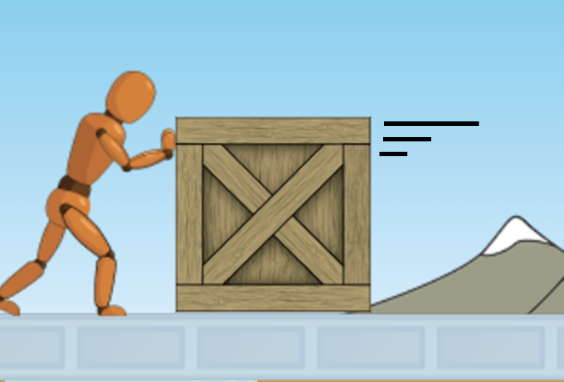
\includegraphics[width=5cm]{physics/figures/unit-4-person-pushing-box.png}
\end{center}

The net force is applied to the box which gets displaced \SI{5}{m} to the left.  What is the net work done on the object? 

\begin{randomizeoneparchoices}[norandomize]
    \choice $-\SI{2}{N\cdot m}$
    \choice $+\SI{2}{N\cdot m}$
    \correctchoice $-\SI{50}{N\cdot m}$
    \choice $+\SI{50}{N\cdot m}$
\end{randomizeoneparchoices}

\clearpage

\question
A box is pushed at a constant velocity across some carpet.  Which of the following statements is wrong?

\begin{randomizechoices}[norandomize]
    \correctchoice Net work is being done to push the box forward.
    \choice The box has a constant momentum.
    \choice The box has a constant kinetic energy.
    \choice The force pushing the box forwards balances the force of friction pushing it back.
\end{randomizechoices}

\question
In which of the following scenarios was the most net work done?

\begin{randomizechoices}[norandomize]
    \choice A net force of \SI{10}{N} is applied to an object as it is displaced \SI{1}{m}.
    \choice A \SI{5}{kg} object's velocity is increased from \SI{1}{m/s} to \SI{3}{m/s}.
    \choice An object's kinetic energy is increased by \SI{20}{N\cdot m}.
    \correctchoice A net force of \SI{5}{N} is applied to an object as it is displaced \SI{5}{m}.
\end{randomizechoices}

\question
The object depicted below has a mass of \SI{5}{kg}.

\begin{center}
    \begin{tikzpicture}[x=0.2cm,y=0.2cm]
        \draw[->,thick] (1cm,0.5cm) -- ++(15,0) node[right] {\SI{15}{N}};
        \draw[->,thick] (0,0.5cm) -- ++(-5,0) node[left] {\SI{5}{N}};
        \draw[fill=lightgray] (0,0) rectangle ++(1cm,1cm);
    \end{tikzpicture}
\end{center}

The forces shown last for 4 seconds. What is the object's change in velocity during that time?

\begin{randomizeoneparchoices}
    \choice \SI{10}{m/s}
    \correctchoice \SI{8}{m/s}
    \choice \SI{40}{m/s}
    \choice \SI{5}{m/s}
\end{randomizeoneparchoices}

\question
The motion map above shows a ball moving to the left during a time interval.

\begin{center}
    \begin{tikzpicture}[scale=0.6]
        \draw[domain=0:10,mark=*,only marks, samples=7,mark size=3.5pt] plot({0.1*\x^2},0);
        \draw[thick, ->] (6,0.8) -- ++(-3,0);
    \end{tikzpicture}
\end{center}

During that time, the net force is \fillin[]\ and the net work done on the ball is \fillin[].

\begin{randomizechoices}[norandomize]
    \choice to the left; positive
    \choice to the left; negative
    \choice to the right; positive
    \correctchoice to the right; negative
\end{randomizechoices}


\question
The velocity vs time graph below shows the motion of a \SI{10}{kg} object.

\begin{center}
\begin{tikzpicture}
    \begin{axis}[height=4.5cm,width=6.5cm,
        axis y line=left,
        axis x line=center,
        ylabel={Velocity (m/s)},
        xlabel={Time (s)},
        ymin=-30,ymax=30,
        xmin=0,xmax=10,
        grid=both,
        ytick={-30,-20,...,30},
        xtick={0,1,...,10},
        x label style={at={(axis description cs: 1,0.5)},anchor=west},
    ]
        \addplot[very thick] coordinates{(0,-20) (4,-20) (4,20) (10,20)};
    \end{axis}
\end{tikzpicture}
\end{center}

What is the object's change in momentum during this time?

\begin{randomizeoneparchoices}[norandomize]
    \choice $+\SI{200}{kg\cdot m/s}$
    \choice $+\SI{5}{kg\cdot m/s}$
    \choice $-\SI{200}{kg\cdot m/s}$
    \correctchoice $+\SI{400}{kg\cdot m/s}$
\end{randomizeoneparchoices}


\question
A cart is pushed across the floor during a time period of 5 seconds.  The net force on the box is shown in the graph below.

\begin{center}
    \begin{tikzpicture}
        \begin{axis}[width=6cm,height=4cm,
            xmin=0,xmax=10,
            ymin=0,ymax=12,
            axis lines=left,
            xlabel={Distance (m)},
            ylabel={Force (N)},
            y label style={rotate=-90},
            xtick={0,1,...,10},
            ytick={0,2,...,12},
            grid=both,
        ]
            \addplot[very thick] coordinates{(0,8)(10,8)};
        \end{axis}
    \end{tikzpicture}
\end{center}

How much power was used to push the box?

\begin{randomizeoneparchoices}[norandomize]
    \choice 0.8 Watts
    \correctchoice 16 Watts
    \choice 40 Watts
    \choice 80 Watts
\end{randomizeoneparchoices}



\question
A man and a woman both push on their own \SI{50}{kg} boxes across the same floor. The man pushes over a distance of 5 meters and then lets go. The woman pushes over a distance of 10 meters and then lets go.  Both the man and the woman push with a force of 200 Newtons. When they let go, the woman's box moves faster. What is a correct explanation of this?

\begin{randomizechoices}[norandomize]
    \choice The woman's box had more acceleration which made the box move faster.
    \choice The woman's box had more net force which made the box move faster
    \choice The woman's box had a greater starting velocity than the man's box
    \correctchoice The woman's force did work over a longer distance giving the box more kinetic energy.
\end{randomizechoices}

\begin{solution}
The work done by the man and woman, respectively, is

\begin{equation*}
    W_1 = F d_1 \qquad W_2 = F d_2
\end{equation*}

where $F = \SI{200}{N}$ is their common force. Since the woman's distance $d_2$ is twice the man's distance $d_1$, the woman does more work on the box. By the work-energy theorem, $W = \Delta \text{KE}$, the woman's box will have more kinetic energy and therefore be moving faster. 
    
\end{solution}

\question
Bo rolls a \SI{3}{kg} bowling ball across the floor while speeding it up to \SI{5}{m/s} in 3 seconds. John rolls the same \SI{3}{kg} bowling ball across the floor while speeding it up to \SI{5}{m/s}. This takes John 4 seconds.  Who uses the most power?

\begin{randomizechoices}[norandomize]
    \correctchoice Bo, because he does the same amount of work in less time. 
    \choice John, because he pushes for a longer time.
    \choice Bo and John use equal power, because they both get the ball up to the same speed.
\end{randomizechoices}




\ifversionKlevel
\question
The graph below shows the net force on a scooter as a function of time. At time $t=0$, the velocity of the scooter is \SI{17}{m/s}. The scooter's mass is \SI{100}{kg}. Find the scooter's final velocity.

\begin{center}
\begin{tikzpicture}
    \begin{axis}[height=4.5cm,width=5.5cm,
        axis lines=left,
        ylabel={Net Force (N)},
        xlabel={Time (s)},
        ymin=0,ymax=1000,
        xmin=0,xmax=6,
        ytick={0,200,...,1000},
        xtick={0,1,...,6},
        grid=both,
        % minor y tick num=1,
        grid=both
    ]
        \addplot[very thick] (0,0) -- (5,800);   
    \end{axis}
\end{tikzpicture}
\end{center}

\begin{randomizeoneparchoices}
    \correctchoice \SI{37}{m/s}
    \choice \SI{20}{m/s}
    \choice \SI{40}{m/s}
    \choice \SI{57}{m/s}
\end{randomizeoneparchoices}

\begin{solution}
We are given the time interval $\Delta t = \SI{5}{s}$, mass $m = \SI{100}{kg}$, and initial velocity $v_i = \SI{17}{m/s}$. These quantities are related by the impulse-momentum theorem, which states 

\begin{equation*}
    F_\text{ave} \Delta t = m(v_f - v_i)
\end{equation*}

If the net force is increasing linearly from 0 to \SI{800}{N}, then the average is \SI{400}{N}:

\begin{equation*}
    F_\text{ave} = \SI{400}{N}
\end{equation*}

Thus we can solve the impulse-momentum theorem for final velocity:

\vspace{-1em}
\begin{align*}
    v_f &= \frac{F_\text{ave} \Delta t}{m} + v_i \\[1ex]
    &= \frac{(\SI{400}{N})(\SI{5}{s})}{\SI{100}{kg}} + \SI{17}{m/s} \\[1ex]
    &= \boxed{\SI{37}{m/s}}
\end{align*}
\end{solution}

\question 
A penguin slides across an icy floor at \SI{4}{m/s}. A strong gust of wind pushes the penguin, increasing her speed to \SI{11}{m/s}. The penguin's mass is \SI{12}{kg}. Calculate the net work on the penguin. 

\begin{randomizeoneparchoices}
    \correctchoice \SI{630}{J}
    \choice \SI{726}{J}
    \choice \SI{96}{J}
    \choice \SI{294}{J}
\end{randomizeoneparchoices}

\begin{solution}
By the work-energy theorem,

\vspace{-1em}
\begin{align*}
    W_\text{net} = \Delta \mathrm{KE} &= \frac{1}{2}mv_f^2 - \frac{1}{2}m v_i^2 \\[1ex]
    &= \frac{1}{2} (\SI{12}{kg}) (\SI{11}{m/s})^2 - \frac{1}{2} (\SI{12}{kg}) (\SI{4}{m/s})^2 \\[1ex]
    &= \boxed{\SI{630}{J}}
\end{align*}
\end{solution}

\question
A conveyor belt in a warehouse operates at 2.6 horsepower. Assuming it operates at 100\% efficiency, how much work is done by the belt in half a second? One horsepower is equal to 746 Watts. 

\begin{randomizeoneparchoices}
    \correctchoice \SI{970}{J}
    \choice \SI{1940}{J}
    \choice \SI{373}{J}
    \choice \SI{130}{J}
\end{randomizeoneparchoices}

\begin{solution}
The belt's power is

\begin{equation*}
    P = \SI{2.6}{hp} = \SI{2.6}{hp} \times \frac{\SI{746}{W}}{\SI{1}{hp}} = \SI{1940}{W}
\end{equation*}

Power is work divided by time, or

\begin{equation*}
    P = \frac{W}{t}
\end{equation*}

So,

\begin{equation*}
    \SI{1940}{W} = \frac{W}{\SI{0.5}{s}}
\end{equation*}

Solving for work, we get

\begin{equation*}
    W = (\SI{1940}{W})(\SI{0.5}{s}) = \boxed{\SI{970}{J}}
\end{equation*}
\end{solution}
\fi


\clearpage

\begingradingrange{myrange} 
\question[2]
The \SI{1000}{kg} car below is moving at \SI{30}{m/s}.


\begin{center}
    \begin{tikzpicture}
        \foreach \i in {0,5,7.5,8.75}{
            \node at (\i,0) {\reflectbox{\twemoji[width=8mm]{automobile}}};
        }
    \end{tikzpicture}    
\end{center}

It comes to a stop in 5 seconds.  What is the average force on the car during this time?

\begin{solutionorbox}[6cm]

\textbf{\color{red} 1 point earned}: For writing the given information and/or invoking the impulse-momentum theorem: \medskip

We know $m = \SI{1000}{kg}$, $\Delta v = \SI{-30}{m/s}$, and $\Delta t = \SI{5}{s}$. \medskip


By the impulse-momentum theorem,

\begin{equation*}
    F_\mathrm{net} \Delta t = \Delta p = m \Delta v
\end{equation*}

\textbf{\color{red} 1 point earned}: For manipulating equation or arrive at the correct answer:

Therefore,

\vspace{-1em}
\begin{align*}
    F_\mathrm{net} &= \frac{m \Delta v}{\Delta t} \\[1ex]
    &= \frac{(\SI{1000}{kg})(-\SI{30}{m/s})}{\SI{5}{s}} \\[1ex]
    &= \boxed{\SI{-6000}{N}}
\end{align*}
\end{solutionorbox}

% \begin{randomizechoices}[norandomize]
%     \correctchoice \SI{6000}{N}
%     \choice \SI{3000}{N}
%     \choice \SI[group-separator={,}]{15000}{N}
%     \choice \SI{1600}{N}
% \end{randomizechoices}

\question[2]
Use the word bank below to complete the following sentences. You may use a word more than once.
\vspace{-1ex}

\begin{center}
\begin{minipage}{0.6\textwidth}
\large
\centering
    Impulse is equal to \\[1ex] \fillin[force][3cm] multiplied by \fillin[time][3cm].

    \vspace{1.5em}
    
    Work is equal to\\[1ex] \fillin[force][3cm] multiplied by \fillin[displacement][3cm].
\end{minipage}%
\fbox{
\begin{minipage}{0.35\textwidth}
\centering
\textbf{\underline{Word Bank}}
\vspace{-1em}
\setlength\columnsep{10pt}
\begin{multicols*}{2}
    acceleration\\
    displacement\\
    kinetic energy\\
    force\\
    gravity\\
    inertia\\
    mass\\
    momentum\\
    position\\
    time\\
    velocity\\
    weight\\    
\end{multicols*}
\end{minipage}}
\end{center}

\begin{solution}

\textbf{\color{red} 1 point earned}: For stating that impulse is the product of force and time.

\textbf{\color{red} 1 point earned}: For stating that work is the product of force and displacement.
\end{solution}


\question[2]
Two identical eggs are dropped from the exact same height. Egg A lands on a concrete floor and breaks. Egg B lands on a pillow and survives. Each egg will lose the same amount of momentum after coming to rest on its surface. Use the impulse-momentum theorem to explain why Egg A breaks while Egg B survives.

\ifprintanswers
\else
\fillwithlines{3cm}
\fi

\begin{solution}

\textbf{\color{red} 1 point earned}: For explaining (in words and/or equations) that the force on the egg at impact is governed by the impulse-momentum theorem: $F_\mathrm{ave} \Delta t = \Delta p$.

 \textbf{\color{red} 1 point earned}: For explaining that the pillow increases the time interval during which the pillow's force on the egg occurs, thus decreasing the magnitude of this force.

 Alternatively, the student gets credit for explaining this in terms of the concrete floor, with a smaller time interval of contact yielding a larger force.
\end{solution}

\vspace*{\fill}

\ifprintanswers
\else
\begin{mdframed}[backgroundcolor=black!10]
    \centering
    \textbf{\small TEACHER USE ONLY}\\[1em]
    \partialgradetable{myrange}[h][questions]
\end{mdframed}
\fi

\ifversionKlevel
\clearpage

\question[2]
A 50-kg little league baseball player slides on the ground to steal home base. Initially he is sliding at \SI{5}{m/s} when he experiences a negative acceleration due to friction and begins to slow down. His kinetic energy vs time graph is shown below.

\begin{center}
    \begin{tikzpicture}
        \begin{axis}[height=6cm,
            width=6cm,
            ymin=0,ymax=700,
            xmin=0,xmax=3,
            ytick={0,100,...,700},
            xtick={0,0.5,...,3},
            axis lines=left,
            ylabel={Kinetic Energy (J)},
            xlabel={Time (s)},
            grid=both,
            clip=false,
        ]
            \addplot[domain=0:2.5,ultra thick,black] {0.5*50*(5 - 100*x/50)^2};
        \end{axis}
    \end{tikzpicture}
\end{center}

Use the information above to calculate the magnitude of the average power dissipated by friction.

\begin{solutionorbox}[12cm]

\textbf{\color{red} 1 point earned}: For using the work-energy theorem to calculate the work done on the player: \medskip

We are given mass $m = \SI{50}{kg}$, initial velocity $v_i = \SI{5}{m/s}$, and a final velocity of $v_f = \SI{0}{m/s}$. 

The net work done by friction on the player is the player's change in kinetic energy:

\begin{align*}
    W_\mathrm{net} = \Delta \mathrm{KE} &= \frac{1}{2}m v_f^2 - \frac{1}{2}m v_i^2 \\[1ex]
    &= \frac{1}{2}(\SI{50}{kg}) \left(\SI{0}{m/s}\right)^2 - \frac{1}{2}(\SI{50}{kg}) \left(\SI{5}{m/s}\right)^2 \\[1ex]
    &= \SI{-625}{J}
\end{align*}

\textbf{\color{red} 1 point earned}: For dividing net work by time to calculate power:

According to the graph, the time interval during which work was done is $\Delta t = \SI{2.5}{s}$. Taking the absolute value, the power is

\begin{align*}
    P &= \frac{\left|W_\mathrm{net}\right|}{\Delta t} \\[1ex]
    &= \frac{\SI{625}{J}}{\SI{2.5}{s}} \\[1ex]
    &= \boxed{\SI{250}{W}}
\end{align*}
\end{solutionorbox}
\fi
\endgradingrange{myrange} 
% \pointsinrange{myrange}



% \hrule\hrule\hrule
% \phantom{.} \hfill {\small \bfseries TEACHER USE ONLY} \hfill \phantom{.}


\end{questions}

\end{document}



\question
What is the average force exerted on a 0.057-kg tennis ball by a racket, assuming that the ball started from rest, that the ball's speed just after impact is \SI{49}{m/s}, and that the ball remained in contact with the racket for 6.1 milliseconds? (Note: There are 1000 milliseconds in one second.)

\begin{solutionorbox}[6cm]
We are given mass, initial velocity, final velocity, and the time interval:

\vspace{-1em}
\begin{align*}
    m &= \SI{0.057}{kg}  \\[1ex]
    v_i &= \SI{0}{m/s} \\[1ex]
    v_f &= \SI{49}{m/s} \\[1ex] 
    \Delta t &= \SI{0.0061}{s}
\end{align*}
\vspace{-1em}

To find the force, we use the impulse-momentum theorem:

\begin{equation*}
    F_\text{net} \Delta t = \Delta p
\end{equation*}

The change in momentum for the ball is

\begin{equation*}
    \Delta p = m (v_f - v_i) = \SI{2.793}{kg m/s}
\end{equation*}

Therefore, the net force on the ball is

\begin{equation*}
    `F_\text{net} = \frac{\Delta p}{\Delta t} = \boxed{\SI{458}{N}}
\end{equation*}
\end{solutionorbox}

\question
If a net force of \SI{-5}{N} is acting on a \SI{10}{kg} object, what will the acceleration of the object be?

\begin{randomizechoices}[norandomize]
    \correctchoice \SI{-0.5}{m/s/s}
    \choice \SI{-2}{m/s/s}
    \choice \SI{-5}{m/s/s}
    \choice \SI{-50}{m/s/s}
\end{randomizechoices}



\begin{randomizechoices}[norandomize]
    \choice \SI{2}{kg}
    \correctchoice \SI{5}{kg}
    \choice \SI{10}{kg}
    \choice \SI{20}{kg}
\end{randomizechoices}






% \question
% A force of \SI{30}{N} is exerted on a 10-kg box at an angle of \ang{40} above the horizontal. The box moves 5 meters to the right. Assuming that the box starts from rest and that there's no friction, what is the final speed of the box?

% \begin{center}
% \begin{tikzpicture}[x=1.4cm,y=1.4cm]
%     \draw (0,0) -- (5.5,0);
%     \draw (2,0) rectangle ++(1.5,1) node[pos=0.5] {\SI{10}{kg}};
%     \draw[dashed] (3.5,0.5) -- ++(1.5,0);
%     \draw[thick,->] (3.5,0.5) -- ++({1.5*cos(60)},{1.5*sin(60)}) node[above] {$\SI{30}{N}$};
%     \draw (4,0.5) arc (0:60:0.5) node[right,pos=0.7] {$\ang{60}$};
% \end{tikzpicture}
% \end{center}

% \begin{randomizechoices}
%     \correctchoice \SI{3.9}{m/s}
%     \choice \SI{12}{m/s}
%     \choice \SI{23}{m/s}
%     \choice \SI{5.5}{m/s}
% \end{randomizechoices}


% \question
% The position vs time graph shown below shows the motion of an object.

% \begin{center}
%     \begin{tikzpicture}
%         \begin{axis}[height=4cm,
%             width=5cm,
%             ymin=0,ymax=5,
%             xmin=0,xmax=3,
%             ticks=none,
%             axis lines=left,
%             ylabel={Position},
%             y label style={rotate=-90},
%             xlabel={Time},
%         ]
%             \addplot[domain=0:2,very thick,black] {4*x - x^2};
%         \end{axis}
%     \end{tikzpicture}
% \end{center}

% The object is experiencing a \fillin[]\ change in momentum, and a \fillin[]\ change in kinetic energy.

% \begin{randomizechoices}[norandomize]
%     \correctchoice negative; negative
%     \choice negative; positive
%     \choice positive; negative
%     \choice positive; positive
% \end{randomizechoices}